%%%%% Dokumentenklasse mit verschiedenen Attributen
\documentclass[a4paper, bibtotocnumbered,liststotoc,12pt,abstracton]{scrartcl}

%%%%% Betriebssystemabh�ngige Eingabedekodierung
\usepackage[T1]{fontenc}
\usepackage[latin1]{inputenc} %% f�r Windows

%%% Python code
\usepackage{listings}             % Include the listings-package
\lstset{language=Python}          % Set your language (you can change the language for each code-block optionally)


%%%%% \usepackage[applemac]{inputenc} %% f�r Mac
\usepackage[ngerman, english]{babel}

%%%% Package to write URLs
\usepackage[colorlinks, linkcolor=blue]{hyperref}
%\usepackage[colorlinks, allcolors=black]{hyperref}


%%%% adjust captions (must be after hyperref)
\usepackage[all]{hypcap}

%%%% Arial
%\usepackage{uarial}
%\renewcommand{\familydefault}{\sfdefault}
%\usepackage{blindtext}

%%%%% Zeilenabstand
\usepackage{setspace}
\onehalfspacing %anderthalbzeilig

%%%%% Mathematik und Symbole
\usepackage{amsmath}
\usepackage{amssymb}
\usepackage{amsthm}

%%%%% Seitenr�nder und Ausrichtung
\usepackage[paper=a4paper,left=30mm,right=25mm,top=25mm,bottom=35mm]{geometry} %define margins..
\geometry{a4paper} % hier auch m�glich 'letter' oder 'a5paper' ... etc.
\usepackage{lmodern}
\usepackage{verbatim}
\setkomafont{sectioning}{\rmfamily\bfseries\boldmath}
\usepackage[usenames,dvipsnames]{color}


%%%%% �berschriften
%\pagestyle{headings} %F�gt �berschrift �ber jeder Seite ein

\usepackage{overcite}

%%%%% Tabellen und Grafiken
\usepackage{booktabs}
\usepackage{tabularx}
\usepackage{array}
\usepackage{graphicx}
\usepackage{rotating}
\usepackage{xtab}
\usepackage{float}

%%%%% Sonstiges

%%%%% Umgebungen f�r S�tze, Propositionen,...
\newtheorem{hyp}{Hypothesis}
\newtheorem*{beweis}{Beweis}
\newtheorem{theorem}{Theorem}
\newtheorem{prop}{Property}

%%%%%%%%%%%%%%%%%%%%%%%%%%%%%%%%%%%%%%%%%%%%%%%%%%%%%%%%%%%%%%%%%%%%%%%
%%%%% BEGIN DOCUMENT %%%%%%%%%%%%%%%%%%%%%%%%%%%%%%%%%%%%%%%%%%%%%%%%%%%%%%%
\begin{document}
\selectlanguage{english}

%%%%%%%%%%%%%%%%%%%%%%%%%%%%%%%%%%%%%%%%%%%%%%%%%%%%%%%%%%%%%%%%%%%%%%%
%% TITLE PAGE %%%%%%%%%%%%%%%%%%%%%%%%%%%%%%%%%%%%%%%%%%%%%%%%%%%%%%%%%%%%%%
\selectlanguage{ngerman}
\begin{titlepage}
\large{Timo Meiendresch}
 \vspace{\fill}
\begin{center}
\Huge{Recurrent Neural Networks for Time Series Forecasting}\\
\large{}
\end{center}
 \vspace{\fill}
\large{Master Thesis (M.Sc. Economics)} \\
\large{Lecturers: Tom Zimmermann and Simon Umbach}\\
\vspace{\fill}\\ Cologne 2019\\
%Cologne
\end{titlepage}
\selectlanguage{english}
%%%% Inhalts-, Abbildungs- und Tabellenverzeichnis
\tableofcontents %f�gt ein Inhaltsverzeichnis ein
%\listoffigures % f�gt ein Abbildungsverzeichnis ein 
%\listoftables % f�gt ein Tabellenverzeichnis ein %\newpage % Seitenumbruch %%%%%%%%%%%%%%%%%%%%%%%%%%%%% Hauptteil %%%%%%%%%%%%%%%%%%%%%%%%%%%%%%%
\newpage
\begin{abstract} 
The year is 2019 A.D. Quantitative research is entirely occupied by Machine Learning (ML). Well, not entirely... One small group of indomitable forecasters still holds out against the invaders. And life is not easy for the ML evangelists who garrison the fortified camps of quantitative research...
\end{abstract}

\section{Introduction}
% Importance of time series forecasting
Time series forecasting is an essential tool in business, economics, and many other disciplines. The ability to accurately predict future values given historic data is of huge importance to 
decision makers. 

% Surge of ML methods 
In recent years, \textbf{Machine Learning (ML)} methods had huge success in many areas of quantitative research. Prominent examples include classification tasks, image processing, or text analysis. ML took many fields by storm and it seems that many quantitative disciplines can benefit from giving in to the AI wave.

% Contrast to time series forecasting
And yet, ML methods are rarely considered in time series forecasting. Research indicated that the performance of ML methods were not able to compete to traditional methods for a long time. Moreover, traditional statistical methods are often easier to implement, computationally cheap, and interpretable. Noteworthy examples include the \textbf{Autoregressive Integrated Moving-Average (ARIMA)} and the various \textbf{Exponential Smoothing (ES)} methods. 
% Notion
Until recently, a widely shared notion was that complex methods for time series forecasting were universally not performing better than traditional ones (e.g. \hyperlink{cite.Hyndman2019}{Hyndman, 2019}). Among others, \hyperlink{cite.M+2018}{Makridakis et al. (2018)} noted just recently that there is only very limited scientific evidence which suggests that artificial neural networks may be a useful tool for time series forecasting. 

\subsubsection*{Paradigm Shift}
% Advances
But, advances in recent years start to challenge this perception. This gradual shift can be traced by a series of forecasting competitions.

% Web Traffic Time Series Forecasting
One notable example is the "Web Traffic Time Series Forecasting" competition hosted by \hyperlink{cite.Kaggle_web}{Kaggle (2017)}. The task was to forecast web traffic for 145,000 wikipedia articles over time. The winning solution by \hyperlink{cite.Arturus_web}{Arturus (2018)} was based on a Long Short-term Memory (LSTM) recurrent neural network which originated in text analysis (\hyperlink{cite.Graves2013}{Graves, 2013}; \hyperlink{cite.S+2014}{Sutskever et al., 2014}). This architecture is often referred to as sequence-to-sequence (seq2seq) model. Along with this seq2seq network architecture, the author incorporated time-specific features to capture the relative position of the observation in time. For example, features were used to indicate the day of the month, or month of the year to capture year-to-year or quarter-to-quarter seasonality. The approach of the model has strong resemblance to the more general implementation of the DeepAR algorithm which is covered in later chapters. 

% M4 competition
To even greater attention came the winner of the most recent version of the M4 competition (\hyperlink{cite.M+2019}{Makridakis et al., 2019}). The M4 competition was the fourth round of a time series forecasting competition with the objective to identify the most accurate forecasting methods. These methods had to produce forecasts for a highly diverse dataset of 100,000 univariate time series from six domains and across six frequencies. Most accurate among 61 contributions was a method by \hyperlink{cite.Smyl2019}{Smyl (2019)} which is a highly complex hybrid of \textbf{recurrent neural network (RNN)} and ES methods. 

% What the results mean and difference between competitions
There is a fundamental difference between the competitions considering the data that were used. Whereas the web traffic series from the Kaggle competition represent a relatively homogeneous dataset, the M4 data are highly diverse and heterogeneous. The former has only one frequency (daily) and series from a very specific area (web traffic), the M4 data come from six rather crude domains (Micro, Macro, Industry, Finance, Demographic, Other) and six different frequencies (Yearly, Quarterly, Monthly, Weekly, Daily, Hourly). The results of the M4 competition showed the potential of recurrent networks even for such a highly diverse dataset, leading to a new surge of interest in the field. 

% Why difference in data is important
\subsubsection*{Local vs. global methods}
Another important aspect, emphasized by the M4 competition, is the transition from local to global methods in time series forecasting. Whereas traditional methods as ARIMA and ES are applied to individual series, ML-based methods are trained using the entirety of available series. These \textbf{local} methods estimate a number of parameters within a model space that is restricted by the respective structure of the model. Because these approaches rely on an explicit model structure with sparse parameters, they are also referred to as \textbf{model-based} (\hyperlink{cite.W+2019}{Wang et al., 2019}). For this, each time series is modeled and trained independently of other series in the data set. Hence, the parameters of the individual model are independent of i) the total number of series in the dataset as well as ii) how similar other series in the dataset are. Both aspects may be important factors in improving accuracy by exploiting general patterns and dependencies. 

Closely related is the emergence and availability of large sets of data, which poses a new kind of forecasting problem, namely to predict huge sets of time series (e.g. \hyperlink{cite.S+2017}{Salinas et al., 2017}). Examples include product sales in online retailers, household energy consumption, or web traffic. In contrast to local models, \textbf{global} methods enable the use of \textbf{cross-series learning}, i.e. general patterns and dependencies can be picked up during the training process for which all available time series are used. This should lead to a general representation of the entire data set. In theory, RNN-based methods should be able to learn across individual series and extract general patterns of the data as well as learn dependency relationships between the individual series. The results of the forecasting competitions imply that this can actually improve forecast accuracy compared to local approaches.

There are various methods based on the idea of cross-series learning, in particular utilizing recurrent networks. The determinants of their performance is a relatively new question into which very little empirical research has so far been done. In theory, RNN should be able to work as a universal function approximator if it is only powerful enough. In practice however, the learnability of RNNs is limited. A typical problem is that they do not converge during training and loss doesn't decrease. This is why these networks are considered to be difficult to train. This is an important factor for practitioners as training a powerful network on such a huge amount of data is computationally expensive. Hence, in context of this project and RNN-based models, there are two main characteristics that should be considered in characterizing the underlying data basis, namely  
\begin{prop}
The total number of individual time series in the underlying data set. How many time series are in the dataset as a whole?
\end{prop}
\begin{prop}
Similarity of the individual time series in the data set. How different are the time series in the dataset?
\end{prop}

Thus far, the models under consideration often neglect property 2 as they focus on rather homogeneous data even though the M4 competition showed that this kind of models could efficiently tackle highly diverse data. Moreover, these methods lack rigorous comparison with previous methods and known data sets for which benchmarks exist. This capstone project investigates the performance of three RNN-based methods on the diverse M4 data for which a wide variety of benchmarks exist. These methods are:
\begin{itemize}
\item \textbf{Deep Autoregressive Recurrent Neural Networks (DeepAR)} - \hyperlink{cite.S+2017}{Salinas et al. (2017)}
\item \textbf{Deep State Space Models (DeepState)} - \hyperlink{cite.R+2018}{Rangapuram et al. (2018)}
\item \textbf{Deep Factor Recurrent Neural Network Model (DF-RNN)} - \hyperlink{cite.W+2019}{Wang et al. (2019)}
\end{itemize}
To evaluate these models I will apply them to the hourly, daily, weekly and monthly data of the M4 competition using the same measures of accuracy. Hence, the performance of the three algorithms can be directly compared to a variety of benchmarks that are available. 

% Heterogeneous data vs. Homogeneous data?
Note that these methods are designed and tested for large sets of related. In contrast, the M4 data consist of highly diverse time series from different domains and different frequencies. To the best of my knowledge, there is no thorough empirical investigation that applies the aforementioned algorithms to the M4 subsets. The primary contribution of this paper is to evaluate these algorithms on the well studied M4 data and compare the results to known benchmarks. 

% Structure / Sectioning 
The paper proceeds as follows. In \hyperref[Definition]{Section \ref{Definition}}, I provide an overview of the project and introduce the performance measures. \hyperref[Analysis]{Section \ref{Analysis}} presents the dataset and algorithms, whereas \hyperref[Methodology]{section \ref{Methodology}} describes the implementation. And lastly, \hyperref[Results]{section \ref{Results}} discusses the results.

\section{Definition}
\label{Definition}
\subsection{Project Overview}
% High-level overview of the project
% Background information such as the problem domain
% Project origin
% related data sets or input data given
In this paper, I compare three RNN-based time series forecasting algorithms with the methods of the well studied M4 competition. For this, I use the same data that were used during the competition and employ the same accuracy measures. The methods of the competition include state-of-the-art approaches as well as traditional methods. 

\subsection{Problem Statement}
% Clearly defines the problem
% Strategy for solving the problem
% Discussion of expected solution
Main goal of this paper is to test the performance of the three  algorithms applied to the M4 data. The algorithms are DeepAR, DeepState, and DF-RNN. Results will be compared to traditional time series methods and modern methods that were part of the competition. Within this setup, I can draw several conclusions about the performance of the three approaches applied to a heterogeneous dataset. While a number of studies focus on the applicability on homogeneous dataset, results of the M4 competition show that the underlying data need not necessarily come from a similar data generating process (DGP) in order to produce very accurate forecasts. 

\subsection{Metrics}
I evaluate the performance of the methods using two measures that were also part of the M4 competition. Forecast measures are still a highly active area of research and there is no consensus on which one is considered to be the best one. Hence, two widely used \textbf{scale-independent errors} were used in the competition. Scale-independent means they are independent of the unit of the time series. Because the competition evaluated accuracy across highly diverse time series with different units, scale-independent measures are required. The two measures are the
\begin{itemize}
\item \textbf{symmetric mean absolute percentage error (sMAPE)}
\item and the \textbf{mean absolute scaled error (MASE)}
\end{itemize}
The \textbf{sMAPE} belongs to the class of percentage errors which are unit-free. One drawback of the measure is that it is infinite (or undefined) if the target variable is zero for any $t$ in the period of interest, and is highly skewed towards extreme values if the target variable is close to zero. The measure is defined as 
\begin{align}
sMAPE = \frac{1}{h} \sum_{t=1}^h \frac{2 \,|Y_t-\hat{Y}_t |}{|Y_t| + |\hat{Y}_t|}
\end{align}
where $Y_t$ is the post-sample value, $\hat{Y}_t$ the estimated forecast, and $h$ the forecasting horizon.

Alternatively, \hyperlink{cite.HK2006}{Hyndman and Koehler (2006)} propose the scaled error measure \textbf{MASE} when comparing forecast accuracy across series with different units. In this case, the absolute error is scaled using the \textbf{Mean Absolute Error (MAE)} from a simple forecast method (either naive or seasonal naive method). The method for seasonal data is defined as: 
\begin{align}
MASE = \frac{1}{h} \, \frac{ \sum_{t=1}^h |Y_t - \hat{Y}_t| }{ \frac{1}{n-m} \sum_{t=m+1}^n |Y_t - Y_{t-m}|},
\end{align}
where $m$ indicates the seasonality of the series. In case of non-seasonal data ($m=1$), $Y_t - Y_{t-m}$ simplifies to $Y_t - Y_{t-1}$ being the naive forecast error. The naive forecast predicts the next value to be equal to the last value $\hat{Y}_{t+1} = Y_t$. This yields the non-seasonal version of the MASE as 
\begin{align}
MASE = \frac{1}{h} \, \frac{ \sum_{t=1}^h |Y_t - \hat{Y}_t| }{ \frac{1}{n-m} \sum_{t=m+1}^n |Y_t - Y_{t-m}|}
\end{align}
In addition to measuring point forecast (PF) accuracy using MASE and sMAPE, prediction interval (PI) accuracy was included in the competition for the first time. For this, the \textbf{Mean Scaled Interval Score (MSIS)} has been used as accuracy measure. Note that there are other widely used measures for PF and PI accuracy, such as the normalized sum of quantile losses for quantiles $p \in \{0.5, 0.9\}$. These measures were used for example in the empirical studies of \hyperlink{cite.R+2018}{Rangapuram et al. (2018)} and \hyperlink{cite.W+2019}{Wang et al. (2019)}. For reference, MSIS and quantile losses are therefore also included in this paper. 

\section{Analysis}
\label{Analysis}
\subsection{Data Exploration}
The M4 dataset consists of 100,000 univariate time series from six domains (Microeconomics, Industry, Macroeconomics, Finance, Demographic, Other) and six different frequencies (Yearly, Quarterly, Monthly, Weekly, Daily). A time series is defined by successive observations in time. Time intervals between observations are equal in this case (equidistant) which means that the time between two observations remains constant for each time series. As the data are from many different fields, units of the observations are different across series and unknown in this dataset.
\begin{table}[h]
\label{fig_m4_overview}
\centering
\textbf{M4 Data  - Overview}\par\medskip
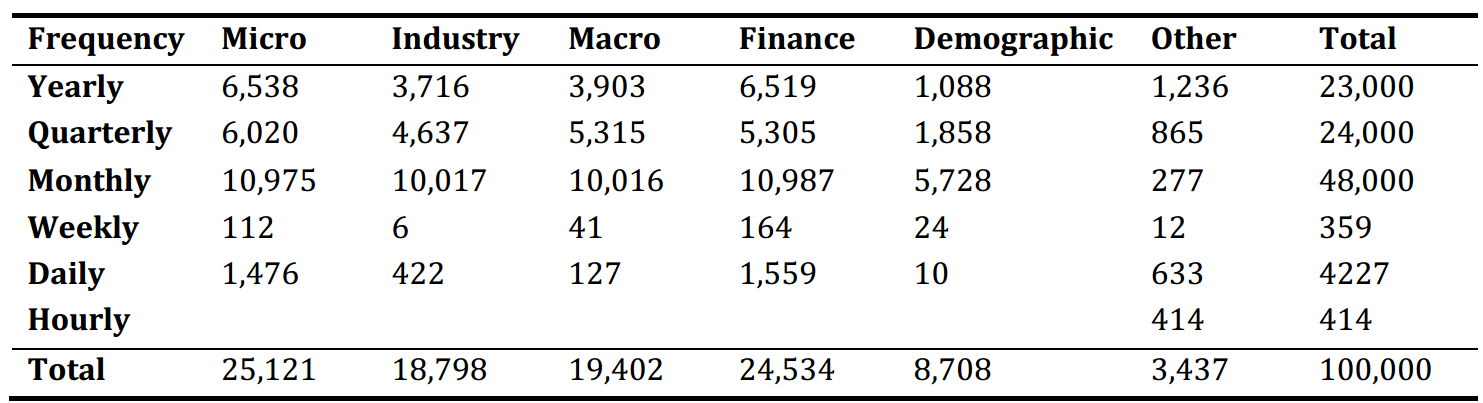
\includegraphics[scale=.58]{../images/M4_data_overview.png} 
\caption{M4 data by domain and frequency.}
\end{table}
The data are a selected subset from a database of more than 900,000 time series and they are of different length. They exhibit common characteristics of time series, such as seasonal patterns, cyclic behavior, as well as trends that the respective model has to capture. Given the behavior of the series, the method has to extrapolate the series into the future. The number of future observations (forecast horizon) to be forecasted is given by
\begin{table}[h]
\label{tab_horizons}
\centering
\textbf{M4 Data - Forecast Horizons}\par\medskip
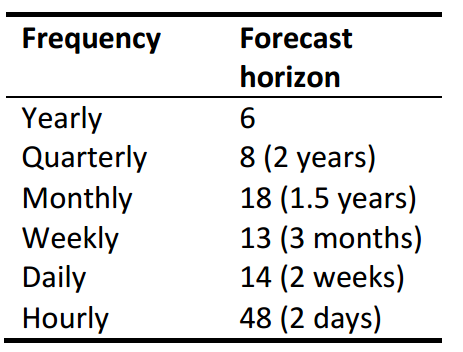
\includegraphics[scale=0.6]{../images/M4_data_forecast_horizon.png} 
\caption{Forecast horizons by frequency of the data.}
\end{table}
A key challenge for the prediction method is the high diversity of the data. Some data exhibit cyclical behavior, up- or downward trends, or varying seasonal patterns. Accurately capturing this behavior to forecast future values is the goal of time series forecasting. 

\subsection{Exploratory Visualization}
As aforementioned, the data are highly diverse. They differ with respect to domain, frequency, and length. For each series there exists a training set as well as an extended test set. The training set consists of a varying number of successive observations in time. The test set includes the same observations but has the additional observations for the forecast horizon. A randomly chosen example series from the hourly M4 data is depicted below: 
\begin{figure}[h]
\label{series338}
\centering
\textbf{M4 Hourly - Series \#338}\par\medskip
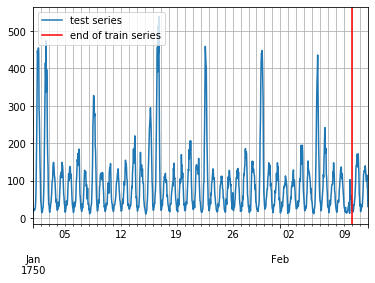
\includegraphics[scale=0.75]{../images/train_test_plot_m4_hourly338.png} 
\caption{Hourly time series 338. The vertical red line indicates where the training data ends and the test set begins.}
\end{figure}

\subsection{Algorithms and Techniques}
% DeepAR
The first of the three algorithms is the \textbf{Deep Autoregressive Recurrent Neural Network (DeepAR)} method, described in \hyperlink{cite.S+2017}{Salinas et al. (2017)}. It is the only built-in time series prediction algorithm in Amazon SageMaker for ML on cloud computing instances. DeepAR uses autoregressive features that are used as the inputs to a recurrent neural network. The RNN uses LSTM cells as default but can also be changed to GRU cells. Previous observations are utilized as inputs which makes this algorithm autoregressive. Examples of this features are day-of-month or week-of-year for weekly data. Which features are included depends on the frequency. 

% DeepState
\hyperlink{cite.R+2018}{Rangapuram et al. (2018)} introduced \textbf{Deep State Space Models (DeepState)}. DeepState combines state space models (SSM) with a recurrent neural network architecture that calculates the optimal parameters for the SSM. The SSM is applied locally to the individual time series. The parameters are determined by a jointly trained RNN using all available data. Hence, this algorithm combines a local method with a global one.

% DF-RNN
Furthermore, I included the \textbf{Deep Factor - Recurrent Neural Network (DF-RNN)} by \hyperlink{cite.W+2019}{Wang et al. (2019)}. This hybrid algorithm uses a local method specific to each time series in the dataset as well as a global RNN, which is trained jointly with the other time series. For now, the only available local method is using another RNN. Hence, the model combines a locally trained RNN with a globally trained RNN. In brief, key characteristics of the three algorithms : 
\begin{itemize}
\item \textbf{DeepAR} - "Pure" global RNN that uses autoregressive features as inputs. 
\item \textbf{DeepState} - Globally trained RNN that determines the best parameters of the local SSM.
\item \textbf{DF-RNN} - Hybrid of a local method that is applied to individual time series and a global RNN that is trained jointly.
\end{itemize}
The training process of the three algorithms uses a fixed window approach. During training, the algorithms extract a sequential number of observations (windows). Each window is a sliced version of the entire time series starting at different points of the series and is of length
\begin{align*}
l_{window} = l_{training} + l_{prediction},
\end{align*}
where $l_{training}$ how many successive training observations are used (training range) and $l_{prediction}$ is the number of successive observations used for the evaluation (prediction range). The prediction range is has the length of the forecast horizon. The default is to use $l_{training} = l_{prediction}$. One window is then fed to the algorithms as one batch. In each epoch a number of batches are fed to the algorithm, where the number of batches per epoch can be varied as well as the number of total training epochs. Stochastic Gradient Descent (SGD) is used to adjust the parameters of the network during the training process. Once the training process is completed, the algorithm uses the parameters of the epoch with the smallest loss as final model. To avoid overfitting, dropout is used by default. Because random numbers are used in this setup, I have fixed them to make the results reproducible.

\subsection{Benchmarks}
In addition to providing a rich dataset across frequencies and domains, a key contribution of the M4 competition is the provision of a rich set of benchmark methods. Not only the metrics of the competition winners but also results for common time series methods, in particular ARIMA and ES, are provided in \hyperlink{cite.M+2019}{Makridakis et al. (2019)} and its additional material. The following discussion will focus on the relative performance of the RNN-based methods with respect to: 
\begin{enumerate}
\item Seasonally adjusted naive predictions (Naive2). This method uses a classical decomposition to deseasonalize the data, then predicts the next value to be equal to the last value and adds the seasonality to this forecast. In general, naive predictions for time series work surprisingly well. 
\item Traditional methods (ARIMA and ES) and the combination benchmark (Comb)
\item Overall winning method of \hyperlink{cite.Smyl2019}{Smyl (2019)}, runner-up by \hyperlink{cite.MM+2019}{Montero-Manso et al. (2019)} as well as the winning method of the frequency under consideration.
\end{enumerate}

\section{Methodology}
\label{Methodology}
\subsection{Data Preprocesing}
The algorithms require the time series inputs in form of a \textbf{JSON Lines}-like format. In Python, this is essentially a dictionary of dictionaries, also referred to as a nested dictionary. Inputs must contain at least the following keys with their respective content: 
\begin{itemize}
\item \texttt{`start`} - Timestamp with the format YYYY-MM-DD HH:MM:SS and the respective frequency of the data
\item \texttt{`target`} - An array of floats or integers that represents the target series of interest. 
\end{itemize}
An example input file takes the form
\begin{lstlisting}[frame=single]
# get first entry in dataset.train
entry = list(dataset.train)[0]

# first entry
entry
>>> {'start': Timestamp('1750-01-01 00:00:00', freq='H'),
 'target': array([605., 586., 586., ..., 521.], dtype=float32)
\end{lstlisting}
Additional keys are optional but often helpful in improving forecast accuracy. Here, the M4 competition does not provide additional covariates to the data. Because there were no dates supplied in the original data, an arbitrary start date is used (i.e. "1750-01-01 00:00:00"). 

\subsection{Implementation}
% Process for which metrics, algorithms, and techniques were implemented with the given datasets or input data has been thoroughly documented. Complications that occured during the coding process are discussed.
To obtain the results of the paper, I use the new \textbf{gluonts} API that is built on the deep learning framework \textbf{MXNet}. I proceed in a similar way for all three algorithms. First, I implement a function that takes in the following arguments: 
\begin{itemize}
\item data - name of the built-in data in gluonts 
\item seed - a seed that fixes the random numbers. Thus, results can be reproduced using the seed from my results table.
\item epochs - Number of epochs a model is trained
\item batches - Number of batches epoch that are used per epoch.
\end{itemize}
\begin{lstlisting}[frame=single]
def deepar(data="m4_weekly", seed=42, epochs=100, batches=50):
    
    dataset = get_dataset(data, regenerate=False)
    mx.random.seed(seed)
    np.random.seed(seed)
    ...
  
    return(output)    
\end{lstlisting}

Applying this function returns a series of accuracy measures. Printing the results leads to 
\begin{lstlisting}[frame=single]
res = deepar(data="m4_weekly", seed=42, epochs=1, batches=50)
pprint(res)

>>> {'MASE': 5.54378962,
 'MSIS': 54.72282354,
 'epochs': 1,
 'sMAPE': 0.12889508,
 'seed': 42,
 'wQuantileLoss[0.5]': 0.09491686,
 'wQuantileLoss[0.9]': 0.07740071}
\end{lstlisting}
One challenge is the instability of the algorithms. Applying the same algrithm twice, keeping all inputs the same (i.e. epochs and batches), leads to different results. This is due to variability in the random numbers used for randomly selecting the series and respective windows. I use seeds to fix the random numbers and make the results reproducible. Note however, that the same seed leads to different random numbers whether a CPU or GPU is used. This issue is reported on github and will probably be fixed in future releases.

To account for the variation between trials I apply the same algorithm using different seeds and keep all else fixed. For this, I use a simple loop that iterates over a range of seeds and applies the respective function repeatedly. My results show the median of three trials.

\begin{lstlisting}[frame=single]
# Loop over a range of seeds
results = []

data="m4_monthly"
epochs=100
batches=50

if __name__ == "__main__":
    for i in range(42, 45):
        print("Seed:", i)
        res = deepar(data, seed=i, epochs, batches)
        pprint(res)
        results.append(res)
\end{lstlisting}
This experimental design makes the results reproducible by using seeds and meaningful by using several trials.

\subsection{Refinement}
One key issue is the diverse nature of the data. There are many adjustable hyperparameters and it seems unlikely that the default values are optimal for all of the four subsets that I use.

%Difference in data 
The number of series within the four subsets range from 359 (M4 weekly) to 48,000 series (M4 monthly). Moreover, the data stems from many different domains and areas. There is no apparent relation between the individual time series. Assuming aforementioned cross-learning by exploiting common patterns and dependencies seems to be difficult in this setting and with this kind of data.

%Hyperparameter
Then again, these algorithms have many adjustable hyperparameters. Some of the seemingly important ones are:
\begin{itemize}
\item context length, 
\item prediction length of the forecasting horizon,
\item epochs,
\item number of batches per epoch,
\item number of RNN layers, 
\item number of RNN cells for each layer, 
\item or dropout rate
\end{itemize}
to mention a few of them. Within the setup of the competition, prediction length is fixed but there are many other moving parts that may influence the prediction accuracy.

A common solution to this problem is to use hyperparameter optimization (HPO) techniques, such as grid search or random search. These HPO techniques essentially run variations of the same algorithm with different hyperparameters to determine the best ones. This is not a feasible option here as some of the models run for as many as thirteen hours per trial. Running different variations multiplies the already high computational costs. To keep computational costs to a bearable level, I start with the default values and adjust the number of epochs if necessary.

\section{Results}
\label{Results}
This section describes the results per frequency, starting from the lowest (hourly) to the highest one (monthly). For every combination of algorithm, data, epochs, and batches, the median result of three trials is included in the table. Trials start with seed 42 because it is "the ultimate answer to life, the universe, and everything..." (\hyperlink{cite.Adams2005}{Adams, 2005}). 
Note that DeepState models are computationally very expensive. Hence, I limited experimentation with DeepState to an acceptable minimum as some models took more than 13 hours of CPU time per trial. Because this algorithm is more stable than the others in terms of results it is unlikely that this alters the conclusions.

\subsection{Model Evaluation and Validation}
\subsubsection*{M4 Hourly}
The hourly subset of the M4 data contains 414 time series. Given forecast horizon is 48, which corresponds to two days. 
\begin{table}[h]
\centering
\textbf{M4 Hourly - Results}\par\medskip
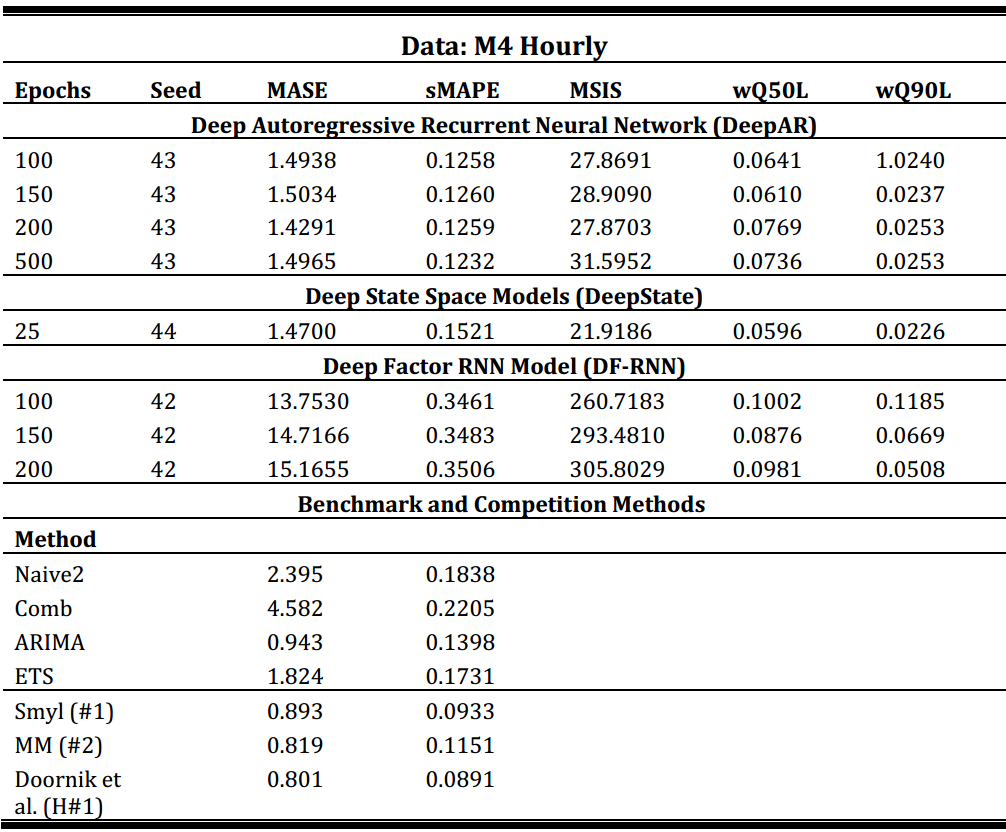
\includegraphics[scale=0.85]{../images/M4_hourly_results.png} 
\caption{Results for hourly M4 data.} \label{m4h_results}
\end{table}
\autoref{m4h_results} illustrates the performance of aforementioned algorithms, respective benchmarks, and winning methods applied to the hourly data of the M4 data. 

It seems that DF-RNN is not able to capture the hourly subset at all. Comparing either MASE or sMAPE to the seasonally adjusted naive forecast (Naive2) shows how bad it works as it is way worse than the seasonally adjusted naive forecast. In addition, its performance is even worse than the standard naive forecast without taking seasonality into account. The naive forecast simply uses the previous value as future forecast (value not shown in the table). 

DeepAR and DeepState show a significantly better performance. They deliver better forecasts than Naive2, Comb, and ETS.  However, the traditional ARIMA method, that is based on modeling the autoregressive behavior of time series, outperforms both models with ease. Additionally, neither of the considered three algorithms comes close to the overall winning method by Smyl that also utilizes RNN. In addition, \hyperlink{cite.MM2019}{Montero-Manso (2019)} and the best hourly method of Doornik and colleagues capture hourly data more precisely than the winning method. 

The performance of DeepAR and DeepState is very similar in this setting but they cannot compete with the traditional ARIMA model nor current state-of-the-art methods. 

\subsubsection*{M4 Daily}
Next, I will discuss the results of the daily subset that are shown in \hyperref[m4_daily_results]{table \ref{m4_daily_results}}. The subset consists of 4227 series and the task is to predict the next 14 observations, i.e. 2 weeks. 

Again, the accuracy of the DF-RNN is nowhere near to being competitive. It first seems as the model converges very slowly for around 200-250 epochs. But after roughtly 250 epochs the loss does not decrease further and the results are quite bad. 
\begin{table}[h]
\label{m4_daily_results}
\centering
\textbf{M4 Daily - Results}\par\medskip
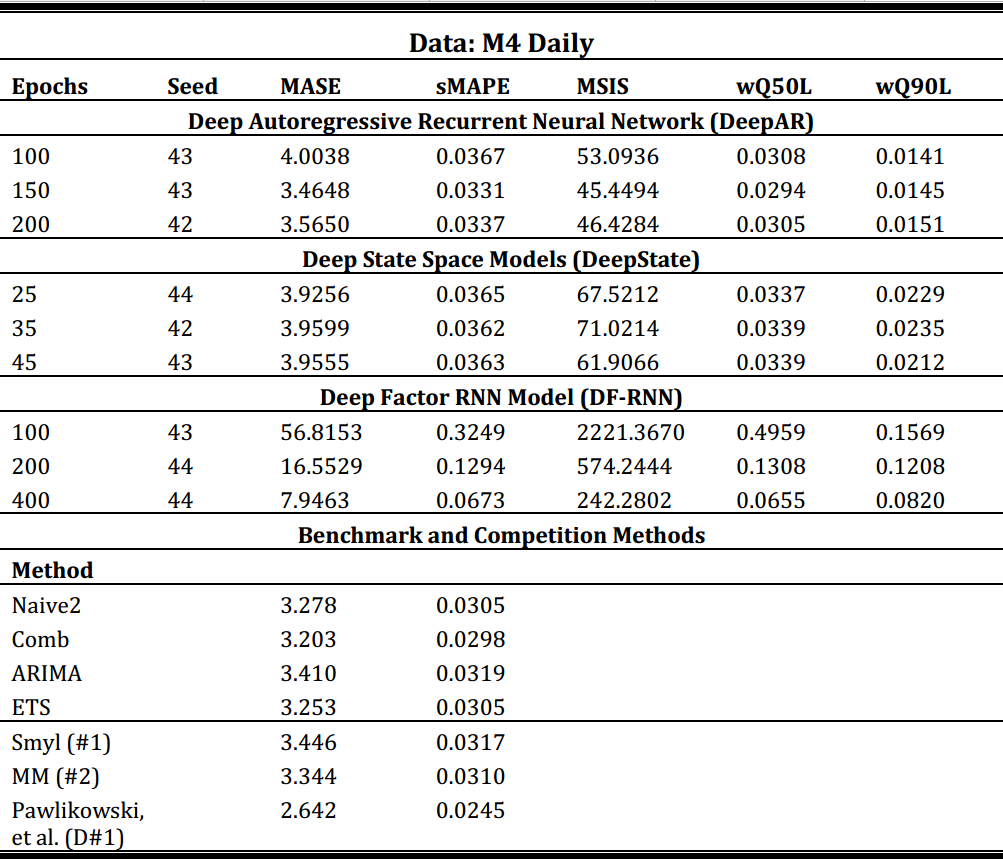
\includegraphics[scale=0.85]{../images/M4_daily_results.png} 
\caption{Results for daily M4 data.}
\end{table}

For DeepAR it seems as if more epochs are required to learn the mapping more accurately. Utilizing 200 epochs and 50 batches per epoch, the loss does not decrease any further after around epoch 100 to 200. DeepAR achieves a similar level of accuracy as ARIMA and the winning method of Smyl. Compared to Naive2, Comb, ETS, as well as the runner-up method of Montero-Manso it performs slightly worse. Note that the Naive2 method performs suprisingly well. It is conceivable that further hyperparameter tuning of DeepAR may lead to further performance improvements to a comparable level of these methods. 

However, there is one outlier method by \hyperlink{cite.P+2019}{Pawlikowski et al. (2019)} whose method performed disproportionately well on the hourly subset of the data. It is not simply better than all other hourly methods, it actually crushes them by a huge margin. Among the overall top ten methods, the method that achieves the second best MASE on the hourly data achieves an MASE of $3.194$. Hence, Pawlikowski's MASE of $2.642$ constitutes a relative performance improvement of staggering $17.28\%$. For comparison, the MASE range of the top ten M4 methods, excluding Pawlikowski, is within $3.194$ and $3.446$. 

For the method of \hyperlink{cite.P+2019}{Pawlikowski et al. (2019)} data are deseasonalized before applying various statistical models, such as ARIMA, simple exponential smoothing, Naive2, Theta method, etc. This yields a series of predictions which are then reseasonalized to restore seasonality. The final forecast is a weighted average of these individual predictions. 

% In-sample forecasting
But, the performance of this model is significantly boosted using in-sample forecasting which may explain the performance edge of the model. This means the authors exploit patterns in the data by searching explicitly for time series with strong correlations. They basically search for time series y that looks similar to x but which is longer. Then, these data points of the longer series y are used to predict future observations of x. In this way, observations are incorporated in the prediction model that actually should not be available. From the perspective of series x, the utilized observations come from the future. This in-sample forecasting is possible because the time series come from different points in time and have different end dates. This can be thought of as having two time series of stock prices, for example Apple (A) and Netflix (N). Series A ends on January 31, whereas series N ends on February 14 of the same year. Your task is now to forecast series A for the time period from February 1 to February 14. Stocks in general exhibit strong correlations and it is a good idea to simply predict stock A to perform in the same way as stock N has performed during the given time period. Unfortunately, future values are usually not available to rely on during prediction which signifies a major problem of this method. 

% The role of stocks and finance time series: strong correlations and these series are (almost) unpredictable.
It should also be noted that $37\%$ of the daily time series originate in the finance domain which are generally considered to be difficult to predict. Using in-sample forecasting vs. out-of-sample forecasting may explain the performance of Pawlikowski's model. Moreover, the comparatively good performance of the Naive2 method may also be an indicator of the presence of series that are difficult to forecast. In the absence of exploitable patterns in the data, predicting the next value to be equal to the previous one is not a bad approach.

Taking this into account, the (almost) untuned version of DeepAR may be closer to the top performing methods than previously thought. It is conceivable that further tuning improves the performance to a competitive level. Further research may be useful to compare DeepAR on other data without the possibility of in-sample forecasting and excluding finance data. 

The presence of overlapping as well as finance data may distort the conclusions drawn from comparing the methods and may also be a reason that the rather simple Naive2 method performs better than all complex RNN methods, including the winning solution by Smyl. 

DeepState performs worse than all other methods, except DeepFactor. In particular, it is not able to replicate the success of the automatic exponential smoothing (ETS) method. This is noteworthy because DeepState uses a complex RNN to fit the best SSM, whereas ETS uses a simpler approach for this.

\subsubsection*{M4 Weekly}
Among the M4 subsets by frequency, the M4 weekly subset is the smallest one with 359 individual time series. The forecast range is 13 which is roughly equivalent to three months or one quarter. 
\begin{table}[h]
\label{m4_weekly_results}
\centering
\textbf{M4 Weekly - Results}\par\medskip
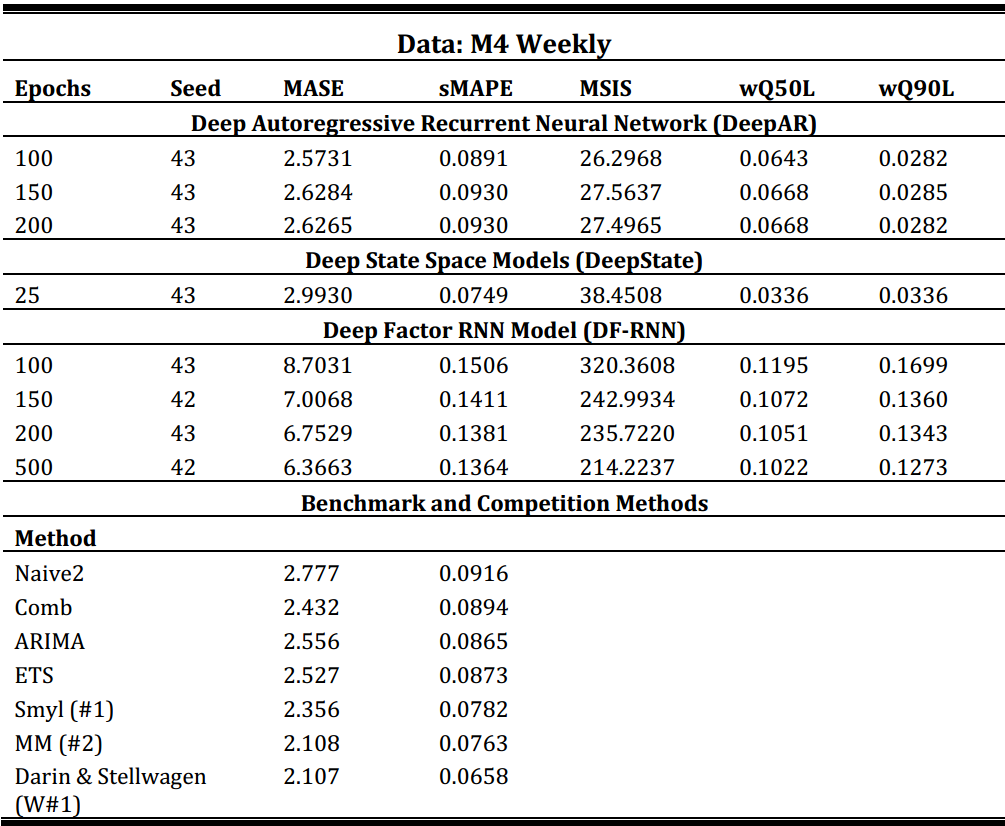
\includegraphics[scale=0.85]{../images/M4_weekly_results.png} 
\caption{Results for weekly M4 data.}
\end{table}
As before, DF-RNN does not fit the data accurately even after increasing the number of training epochs to 500. Because training loss does not decrease further after around 250 epochs and due to the fact that gluonts selects the model with the minimum training loss, another increase in training epochs is unlikely to lead to improve the model's accuracy. 

Applying DeepAR on the weekly subset produces forecasts that are more accurate than the Naive2 method and comparable to the traditional methods as well as the combination benchmark. Comparing the performance to the overall winner of Smyl, DeepAR produces acceptable results. Further improvements by using model tuning or additional features are conceivable. However, the leading methods of Darin and Stellwagen as well as runner-up of Montero-Manso are more accurate relying on local methods. 

The performance of DeepState is again slightly worse than DeepAR but also worse than the Naive2 benchmark. As before, it is quite surprising that the DeepState model does not produce results of similar quality than  ETS, which also uses SSM.

\subsubsection*{M4 Monthly}
The last subset includes the monthly data of the M4 competition. It contains 48,000 time series and is the largest subset of all frequencies. 
\begin{table}[h]
\label{m4_weekly_results}
\centering
\textbf{M4 Monthly - Results}\par\medskip
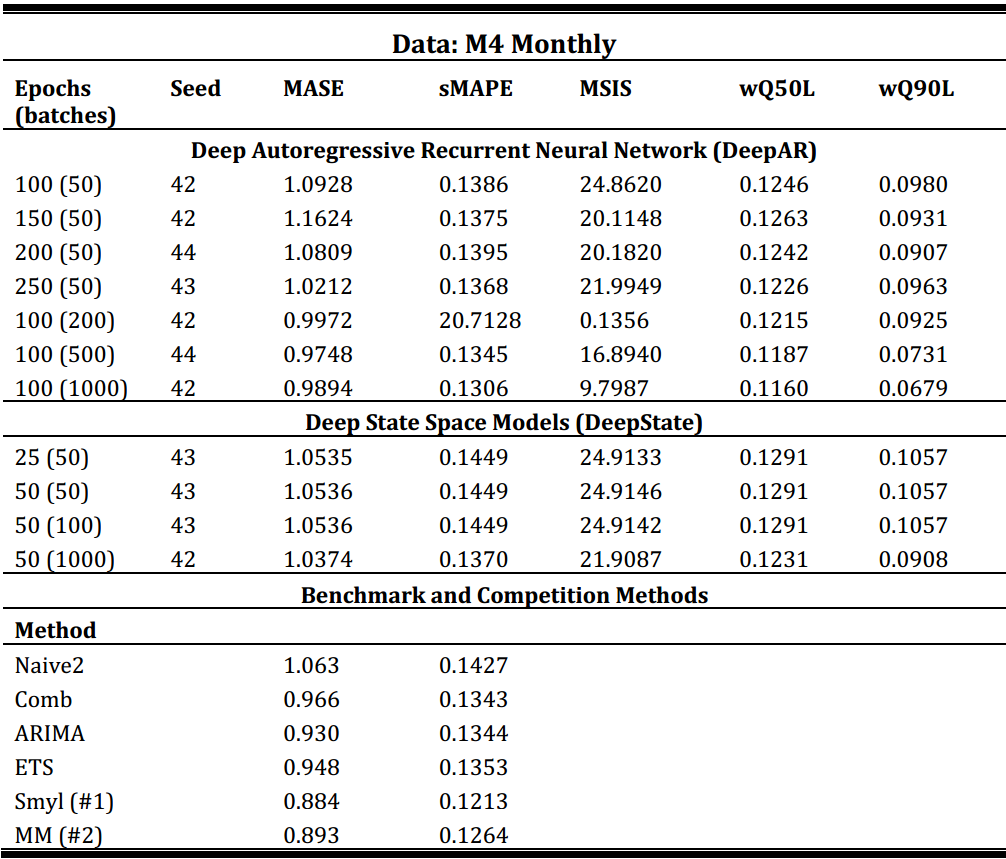
\includegraphics[scale=0.85]{../images/M4_monthly_results.png} 
\caption{Results for monthly M4 data.}
\end{table}
DF-RNN failed again to produce accurate results using default values as well as experimenting with number of epochs, and batches per epoch (not shown in the table).

The DeepAR algorithm produces forecasts that are comparable to the Naive2 and Comb benchmark. Using 100 epochs and 1000 batches per epoch leads to acceptable results but are not an improvement over traditional methods such as ARIMA or ETS. Compared to the overall winning method of Smyl, which was also the most precise method on the monthly subset, there are still considerable performance differences. Because the dataset is really big, a more powerful network (i.e. additional layers) may improve accuracy even further.
It should be noted that there are some convergence issues with the algorithm for smaller batches. It may be the case that the dataset is too large or too diverse to be used with only 50 training examples per epoch. As a result the training loss did not decrease continuously for batch sizes below 200.

Another familiar finding are the results for the DeepState algorithm. Forecast results are slightly worse than DeepAR and slightly better than the Naive2 benchmark. Furthermore, the performance quality is inferior to traditional methods as well as the competition winners. 

\subsection{Conclusion}
% Data Issue
% Homoegeneous vs. Heterogeneous data <- DeepAR may outperform on a homogeneous dataset, what about DeepState? Outperform other M4 methods?
In the course of this project I applied three RNN-based algorithms (DeepAR, DeepState, and DF-RNN) to subsets of the M4 dataset and compared their performance to the competition methods. While I was able to answer how the algorithms performed on the M4 subsets, some questions remain and even more questions were raised.

1) A first implication is that DF-RNN has some major flaws of unknown origin. This makes it unusable for now until they are solved. Note that the authors used a different set of measures and datasets which made a direct comparison difficult. Applying the method to the M4 data with known benchmarks reveals that there are some serious issues with this approach or its implementation. Further research why this method does not deliver the desired results is necessary.


2) The untuned DeepAR algorithm yields accurate predictions that are comparable to traditional methods for some frequencies but not as good as the state-of-the art methods of the competition. It is conceivable that the use of additional features (covariates) or hyperparameter optimization can improve its performance to a competitive level. Unlike most of the competition methods, such as the winning method by Smyl, it can be used "out-of-the-box" by practitioners using either gluonts or AWS SageMaker's built-in version. This increases the value of DeepAR tremendously. Also, the performance may be limited due to the diverse nature of the M4 data. Applying the method to a homogeneous dataset may improve its performance beyond local methods. Comparing its performance on a set of highly related data to the M4 methods may be a rewarding topic for future research.

3) DeepState produces forecasts that are significantly worse than DeepAR and the benchmarks of the competition. However, it seems that DeepState captures at least some of the broad patterns of the data. Additional research into why this algorithm does not fully capture the underlying process may help in solving its issues. Another interesting question is why this global approach does not lead to comparable results as the local ETS method. Both methods use SSM but the selection process of DeepState is global, whereas ETS uses a local statistical one.

4) A shared problem for the algorithms may be the suboptimal choice of hyperparameters. For now, training neural networks seems more like an art than a science. Often, the training process is dominated by trial and error. In the case of RNNs, this seems particularly true as some networks simply won't converge without obvious reasons. The choice of optimal values seems generally difficult. Possible future research  into how this process can be automated without running several variations of this model may help to save computational costs, time, and improve accuracy.

5) Finally, the M4 data are highly diverse with respect to their underlying data-generating process.  They are taken from various domains and across frequencies. The heterogeneous nature may have affected the performance of the algorithms in a negative way. Using a homogeneous dataset for the analysis of the RNN algorithms may yield completely different results and rankings than the M4 competition. In theory, this should improve the learnability of the underlying process. Comparing the global RNN methods with the M4 methods (local and global) can lead to interesting insights into the performance differences between local and global methods. It is likely that global methods outperform local methods only in settings with a lot of similar series. More empirical studies into how many series are required and to what degree the series should be related are necessary. In order to do this it may also be helpful to quantify the degree of similarity between time series in a dataset.

6) Whereas Smyl's method was able to outperform other methods even on such a highly diverse dataset, the introduced RNN algorithms did not. Note that the implementation of Smyl's approach is highly and customized to the M4 data. It cannot be easily reproduced or applied to other datasets for now. Why no other modern RNN algorithm could replicate his results remains a key question. It seems that for now traditional forecasting methods remain important tools in the toolkit of time series forecasters as no out-of-the-box RNN method seems to be able to replace them. If or in which particular area or forecasting they will fit in remains an open question.

% Data Issue
% How does this influence the analysis and conclusions
% Note that there may be the possibility that very complex methods 
%%%%%%%%%%%%%%%%%%%%%%%%%%%%%%%%%%%%%%%%%%%%%%%%%%%%%%%%%%%%%%%%%%%%%%%%%%%%%%%%%%%%%%%%%%%%%%%%%%%
%%%%%%%%%%%%%%%%%%%%%%%%%%%%%%%%%%%%%%%%%%%%%%%%%%%%%%%%%%%%%%%%%%%%%%%%%%%%%%%%%%%%%%%%%%%%%%%%%%%


%%%%%%%%%%%%%%%%%%%%%%%%%%%%%%%%%%%%%%%%%%%%%%%%%%%%%%%%%%%%%%%%%%%%%%%%%%%%%%%%%%%%%%%%%%%%%%%%%%%
%%%%%%%%%%%%%%%%%%%%%%%%%%%%%%%%%%%%%%%%%%%%%%%%%%%%%%%%%%%%%%%%%%%%%%%%%%%%%%%%%%%%%%%%%%%%%%%%%%%


%%%%%%%%%%%%%%%%%%%%%%%%%%%%%%%%%%%%%%%%%%%%%%%%%%%%%%%%%%%%%%%%%%%%%%%
%% Anhang %%%%%%%%%%%%%%%%%%%%%%%%%%%%%%%%%%%%%%%%%%%%%%%%%%%%%%%%%%%%%%
%%%%%%%%%%%%%%%%%%%%%%%%%%%%%%%%%%%%%%%%%%%%%%%%%%%%%%%%%%%%%%%%%%%%%%%
%% LITERATURE %%%%%%%%%%%%%%%%%%%%%%%%%%%%%%%%%%%%%%%%%%%%%%%%%%%%%%%%%%%%%

% View complete list of literature in database
%\nocite*

% List of references
\newpage
%\bibliography{dateiname.bib}
\bibliographystyle{plain}
 \begin{thebibliography}{------}
%alphabetisch sortieren

	\bibitem{Adams2005}
Adams, Douglas. "The Hitchhiker's Guide to the Galaxy." Del Rey Books. 2005

	\bibitem{Arturus_web}
Arturus (2018). "How it works." Retrieved from \url{https://github.com/Arturus/kaggle-web-traffic/blob/master/how_it_works.md}

	\bibitem{Graves2013}
Graves, Alex. "Generating sequences with recurrent neural networks." \textit{arXiv preprint arXiv:1308.0850 (2013).}

	\bibitem{Hyndman2019}
Hyndman, Rob J. "A brief history of forecasting competitions." \textit{International Journal of Forecasting (2019)}.
	
	\bibitem{HK2006}
Hyndman, Rob J., and Anne B. Koehler. "Another look at measures of forecast accuracy." \textit{International journal of forecasting 22.4 (2006): 679-688.}

	\bibitem{Kaggle_web}
Kaggle (2019). "Web Traffic Time Series Forecasting." Retrieved from \url{https://www.kaggle.com/c/web-traffic-time-series-forecasting}

	\bibitem{M+2018}
Makridakis, Spyros, Evangelos Spiliotis, and Vassilios Assimakopoulos. "Statistical and Machine Learning forecasting methods: Concerns and ways forward." \textit{PloS one 13.3 (2018):
e0194889.}

	\bibitem{M+2019}
Makridakis, Spyros, Evangelos Spiliotis, and Vassilios Assimakopoulos. "The M4 competition: 100,000 time series and 61 forecasting methods." \textit{International Journal of Forecasting
(2019).}

	\bibitem{MM+2019}
Montero-Manso, Pablo, et al. "FFORMA: Feature-based forecast model averaging." \textit{International Journal of Forecasting (2019).}

	\bibitem{P+2019}
Pawlikowski, Maciej, and Agata Chorowska. "Weighted ensemble of statistical models." \textit{International Journal of Forecasting (2019).}

	\bibitem{R+2018}
Rangapuram, Syama Sundar, et al. "Deep state space models for time series forecasting." \textit{Advances in Neural Information Processing Systems}. 2018.

	\bibitem{S+2017}
Salinas, David, Valentin Flunkert, and Jan Gasthaus. "DeepAR: Probabilistic forecasting with autoregressive recurrent networks." \textit{arXiv preprint arXiv:1704.04110 (2017).}

	\bibitem{Smyl2019}
Smyl, Slawek. "A hybrid method of exponential smoothing and recurrent neural networks for time series forecasting." \textit{International Journal of Forecasting (2019).}

	\bibitem{SE+2019}
Spiliotis, Evangelos, et al. "Are forecasting competitions data representative of the reality?." \textit{International Journal of Forecasting (2019).}

	\bibitem{S+2014}
Sutskever, Ilya, Oriol Vinyals, and Quoc V. Le. "Sequence to sequence learning with neural networks." \textit{Advances in neural information processing systems. 2014.}

	\bibitem{W+2019}
Wang, Yuyang, et al. "Deep Factors for Forecasting." \textit{arXiv preprint arXiv:1905.12417 (2019).}

 \end{thebibliography}


%%%%%%%%%%%%%%%%%%%%%%%%%%%%%%%%%%%%%%%%%%%%%%%%%%%%%%%%%%%%%%%%%%%%%%%
%% EIDESSTATTLICHE ERKL�RUNG  %%%%%%%%%%%%%%%%%%%%%%%%%%%%%%%%%%%%%%%%%
%\newpage
%\selectlanguage{ngerman}
%\section*{Eidesstattliche Erkl�rung}
%Hiermit versichere ich, dass ich die vorliegende Arbeit selbstst�ndig und ohne die Benutzung anderer als der angegebenen Hilfsmittel angefertigt habe. Alle Stellen, die w�rtlich oder sinngem�� aus ver�ffentlichten und nicht ver�ffentlichten Schriften entnommen wurden, sind als solche kenntlich gemacht.\\
%\\
%K�ln, den \today
%\\
%Unterschrift
%\selectlanguage{english}
\end{document}
